\section{Relational VS NoSQL databases}

\subsection{About Relational databases}
Relational databases use SQL as their query language.
Relational databases (RDBS) have a clear structure. There is DB, then table and data \parencite{web:MSDatabases}. Database is collection of tables and table is collection of data. Schema is enforced, meaning we have strict data types and requirements where data needs to go.

Every table has fields (columns) and records (rows). Every record has the same number of fields unlike NoSQL.

To improve SQL performance, normalisation is performed. With this, one table is broken apart to multiple tables with primary keys and foreign keys \parencite{kohler2018sql}
\newline
Types of relations:
\begin{itemize}
  \item One to one,
  \item many to many,
  \item one to many,
  \item many to one.
\end{itemize}

\subsection{About NOSQL}
Mongo has the structure of: database, collection, documents. Database can have multiple collections and collection can have multiple documents \parencite{web:AboutMongo}. As name suggests, NoSQL means no schema. That means collection can have documents with different sizes inside.
\newline
NoSQL is flexible ${\xrightarrow{}}$ you can add new data to one document and that one document would be different than others\parencite{web:MongoNoSQL}.
\newline
NoSQL does not have relations. They can be implemented (on software level) but they are not enforced with managment system. Due to this, if the data changes, you need to do multiple updates.

\subsection{Cap theorem}
Stands for:
\newline
C - Consistency - data is the same across the database
\newline
A - Availability - as the data is written, it is replicated to other nodes
\newline
P - Partition tolerance - if node goes offline, how can it be replaced
\newline
\parencite{khazaei2016choose}

\begin{figure}[H]
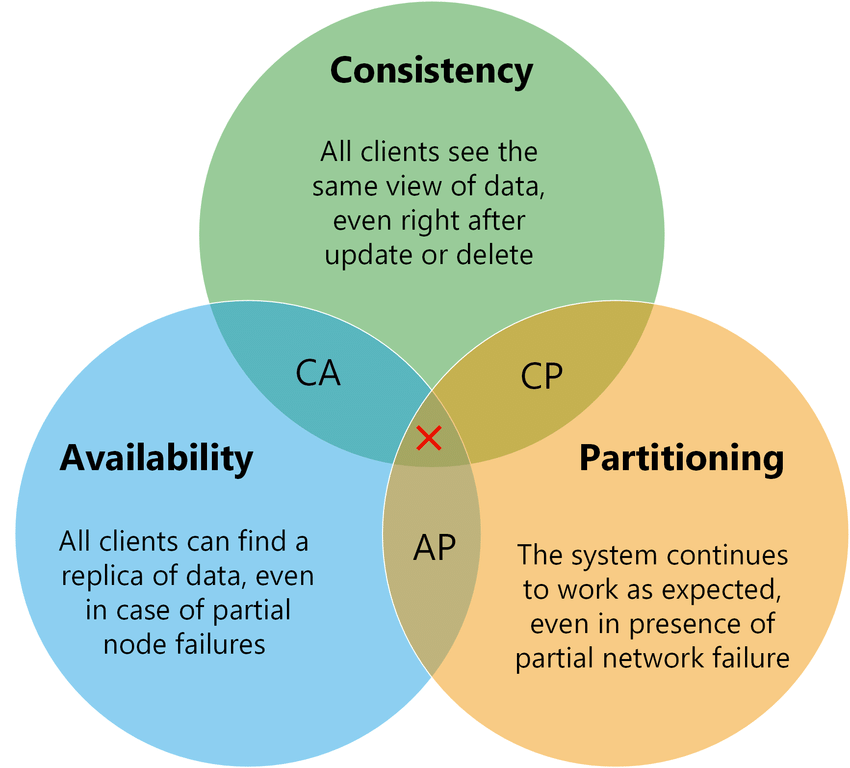
\includegraphics[scale=0.45]{img/CAP.jpeg}
\centering
\caption{CAP theorem representation}
\end{figure}

MongoDB goes under CP, that meaning it is consistent and it has partition tolerance. This is achieved by MongoDB having primary node who receives all the writes and secondary nodes replicate the data after it has been written to primary (consistency). If primary node goes offline, secondary nodes can take over (partition tolerance). MongoDB does not have availability (or HA - high availability) due to it having one master node. So if master node goes offline it takes some time for voting process to be accomplished.

MySQL (relational database) would be CA. Data is written only to one node at the time, this is resulting in consistency. All of the data is also replicated to another node which is resulting in availability. But if master node goes down there is no partitioning in place.

Cassandra on the other hand, is classified as AP. All of the nodes are independent, that is preventing it to have consistency. But due to them not having a master node, read/write can be done from any node and this is resulting in high availability. Nodes are also copying data across to other nodes, this is resulting data (partition) tolerance.
\parencite{web:IBMCAP}

\subsection{Pros for SQL}
\begin{itemize}
  \item uses schemas ${\xrightarrow{}}$ more fixed structure
  \item relations ${\xrightarrow{}}$ no duplicate data, only update once
  \item data is distributed across multiple tables
  \item scaling is vertical
\end{itemize}

\subsection{Pros for NoSQL}
\begin{itemize}
  \item no schema ${\xrightarrow{}}$ data structure can change
  \item relations are not common ${\xrightarrow{}}$ not querying relations 
  \item data is nested in collections together
  \item can scale horizontal and/or vertical
  \item great performance for mass requests
\end{itemize}

\subsection{Scaling}
Scaling can be done in two ways \parencite{cattell2011scalable}
\newline
Horizontal:
\begin{itemize}
    \item add more servers (nodes) and merge data into one DB
    \item data is split across across the servers
\end{itemize}
Vertical:
\begin{itemize}
    \item add more power (upgrade hardware) to existing server 
    \item there is limit of to where you can scale
\end{itemize}



\subsection{Which one is better: SQL or NoSQL}
At the end, it depends on the scenario that we are in. Based on the CAP theorem, lets consider 3 cases:
\begin{itemize}
  \item Consistency and availability (CA)
      \begin{itemize}
        \item This would be for financial institutions, where data needs to be in sync as well as the same.
      \end{itemize}
  \item Consistency and partition tolerance (CP)
      \begin{itemize}
        \item This would be for e-commerce websites where data needs to be consistent and can operate even if node fails. 
      \end{itemize}
  \item Availability and partition tolerance (AP)
      \begin{itemize}
        \item This would be for social media services (like Facebook) where data can be out of sync for some time.
      \end{itemize}
\end{itemize}

Since there is not a clear winner, we can use what is the best for companies use case. Lets use Facebook as an example. They have social media which could be AP, marketplace could be CP and transactions on the site itself which are CA. With this, a company like Facebook can use SQL or NoSQL with correct CAP use case when needed. 
\newline
To have a better representation on how data would be stored in data center, have a look on appendix A1-data centers.